\documentclass[journal]{IEEEtran}

\usepackage{cite}

\usepackage{amsmath,amssymb,amsfonts}
\usepackage{algorithm}
\usepackage{graphicx}
\usepackage{textcomp}
\usepackage{xcolor}
\usepackage{booktabs}
\usepackage{multirow}
\usepackage{array}
\usepackage{subfig}
\usepackage{geometry}
\usepackage{algpseudocode}

\algrenewcommand\algorithmicrequire{\textbf{Input:}}
\algrenewcommand\algorithmicensure{\textbf{Output:}}


\def\BibTeX{{\rm B\kern-.05em{\sc i\kern-.025em b}\kern-.08em
    T\kern-.1667em\lower.7ex\hbox{E}\kern-.125emX}}

\begin{document}

\title{Distributed Collapsed Gibbs Sampling for LDA on Spark}

\author{\IEEEauthorblockN{Agnieszka Ciborowska}\\
\IEEEauthorblockA{\textit{Department of Computer Science} \\
\textit{Virginia Commonwealth University}}}


\maketitle

\begin{abstract}
The report describes distributed collapsed Gibbs sampling for widely used latent Dirichlet allocation (LDA) model implemented on Spark. The algorithm distributes dataset into $P$ partitions and performs local LDA on each partition, for each document independently. Every $n^{th}$ iteration, local LDA models, that were trained on distinct partitions, are combined to assure the model ability to converge. The approach demonstrates comparable performance in the final model quality to the sequential LDA, and achieves significant speedup for large datasets.
\end{abstract}


\begin{IEEEkeywords}
Spark, LDA, collapsed Gibbs sampling
\end{IEEEkeywords}


\section{Introduction}
The advent of the era of big data, when the amount of the produced information increases every day, created many new possibilities for machine learning, but also arose equally important challenges on how to process and analyzed very large datasets efficiently with respect to memory limitations and computational time. One of the many methods that are currently facing this issue, is commonly used latent Dirichlet allocation model proposed by Blei et al.~\cite{blei2003latent}. LDA is a three-level hierarchical Bayesian model designed to discover latent topics in document corpora. The main idea of the model is to represent each document as a random mixture of topics, where each topic is, in turn, modeled by a distribution over words. LDA model can be built using either variational inference or MCMC methods, and both approaches has some advantages and disadvantages. The main leverage of using variational inference is significantly lower computational time, but for the price of possibly inaccurate inference. In the case of MCMC methods, one gains accuracy, at the cost of computational complexity, causing these methods to be  inapplicable for large datasets.

This report introduces a distributed implementation of an MCMC method, a collapsed Gibbs sampling, for LDA on Spark. The approach follows the hypothesis of weak dependency between variables as the number of variables is greatly larger than number of cores used for parallelization\cite{newman2009distributed}, thus it allows to distribute data into $P$ partitions and perform LDA locally. 

To summarize, the contributions of this report are:
\begin{itemize}
\item implementation of a collapsed Gibbs sampling for LDA on Spark, referred further as Spark-LDA,
\item evaluation of the effectiveness of the Spark-LDA model for latent topic discovery task,
\item evaluation of the influence of Spark-LDA's parameters on the model performance and execution time.
\end{itemize}
The organization of this report is as follows. Section \ref{sec:lda} briefly review plain LDA model and collapsed Gibbs sampling procedure, while Section~\ref{sec:slda} provides a detailed description on the distributed LDA implementation using Spark. In Section~\ref{sec:exp}, the report provides the evaluation results of the distributed model and compares them to the sequential algorithm. Finally, Section~\ref{sec:conclusion} concludes the report and outlines plan for future work.

\section{Latent Dirichlet Allocation}
\label{sec:lda}
Before describing the details of Spark-LDA, I briefly review the standard LDA model, illustrated in Figure~\ref{fig:lda} using plate notation.  LDA models each of $D$ documents as a mixture over $K$ latent topics, where each topic is a multinomial probability distribution over a vocabulary of $V$ words. Generative process of creating a new document $j$ can be characterized as follows:
\begin{itemize}
\item draw a mixing proportion $\theta_{k|j}$ from a Dirichlet with parameter $\alpha$,
\item for the $i^{th}$ word in the document, first draw a topic assignment $z_{ij}$, where topic $k$ is chosen with probability of $\theta_{k|j}$, and then value $w$ of word $x_{ij}$ is drawn from the $z_{ij}$ topic with probability $\phi_{w|k}$, where $\phi_{w|z_{ij}}$ is drown from a Dirichlet prior with parameter $\beta$.
\end{itemize}
The above description of the generative process is equivalent to:
$$
\theta_{k|j}\sim Dir(\alpha) \quad \phi_{w|k}\sim Dir(\beta)
$$
$$z_{ij}\sim \theta_{k|j} \quad  x_{ij}\sim \phi_{w|z_{ij}}
$$
where $\alpha$ and $\beta$ are fixed Dirichlet priors.

\begin{figure}
\centering
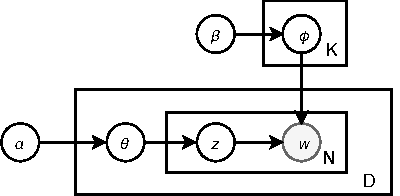
\includegraphics[scale=0.9]{plots/LDA.pdf}
\caption{Graphical model for LDA. Observed variable $w$ is shaded.}
\label{fig:lda}
\end{figure}

Given the observed words $\textbf{x}=\{x_{ij}\}$, the task is to compute the posterior distribution over the latent variables $\texttt{z}$, $\theta$ and $\phi$. The two most frequently applied inference procedures are based on either using variational methods\cite{blei2003latent} or Markov chain Monte Carlo (MCMC) methods \cite{griffiths2004finding}. This report focuses on the latter, more specifically, on a collapsed Gibbs sampling inference procedure for LDA, proposed by Griffiths and Steyvers\cite{griffiths2004finding}. The collapsed Gibbs sampling samples the latent variable $\texttt{z}$ with $\theta$ and $\phi$ integrated out. In this setup the conditional probability of $z_{ij}$ is given by:
$$
p(z_{ij}=k|z^{\lnot ij}, x, \alpha, \beta) = \dfrac{c_{k,m,\cdot} + \alpha}{N_{j}^{\lnot i}+K\alpha} \frac{c_{k,\cdot,n} + \beta}{c_{k,\cdot,\cdot} + V\beta}
$$ 
where $\lnot ij$ denotes word $i$ in document $j$ that is excluded in the count values and $c_{k,m,n}$ represents the number of times topic $k$ is assigned to word $n$ in document $m$. Missing index value for $c_{k,m,n}$ (e.g. $c_{k,\cdot,n}$) denotes summing over that index (e.g. $c_{k,\cdot,n} = \sum_{m=1}^{M} c_{k,m,n}$).

Implementation of a sequential collapsed Gibbs sampler for LDA is straightforward as it operates on a set of count values, $c_{k,\cdot,m}$, $c_{k,m,\cdot}$ and $c_{k,\cdot,\cdot}$. The algorithm starts by randomly assigning a topic to a word in a  document, updating the count values accordingly, and performs loop over the number of iterations to reassign a topic to a word according to the conditional probability. The outline of LDA collapsed Gibbs sampling is presented in Algorithm \ref{alg}.
 \begin{algorithm}
\caption{Gibbs sampling}
\label{alg}
\begin{algorithmic}
\scriptsize
\Require latent variable $z^{(0)} = \langle z_1^{(0)},...,z_k^{(0)}\rangle$
\State \textbf{begin}
   \ForAll  {$t = 1 $ to $T$}
      \ForAll  {$i = 1$ to $k$}
         \State $z^{(t+1)}_i \sim P(Z_i | z_1^{(t+1)},...,z_{i-1}^{(t+1)},z_{i+1}^{(t)},...,z_k^{(t)})$
      \EndFor 
   \EndFor
\State \textbf{end}
        \end{algorithmic}
    \end{algorithm}

\section{Distributed inference for LDA}
\label{sec:slda}
Although LDA with collapsed Gibbs sampling has been in common use, due to its high computational complexity, this method it not applicable for processing large document corpora. Additionally, obtaining the speedup through paralellization is not trivial as collapsed Gibbs sampling is a strictly sequential process that uses the current state of all but one variable to sample new topic assignment $z_{ij}$. This section introduces an approximate collapsed Gibbs sampling procedure for LDA, where data is distributed over distinct processors on Spark.

\subsection{Distributed LDA on Spark}
To distribute the computations, this study follows the hypothesis proposed by Newman et al.\cite{newman2009distributed} and assumes that since the number of words in a document is typically larger than the number of processors, the dependency between topic assignment $z_{ij}$ and $z_{i'j'}$ is weak, thus the sequential sampling requirement can be relaxed and the LDA model can be trained and tested in a distributed environment. 

The main idea of Spark-LDA algorithm is shown in Algorithm~\ref{alg2}. After random initialization, each document $d$ is mapped to a record containing document identifier, sparse bag-of-words representation of the document's content and the count value of $c_{k,d,\cdot}$ corresponding to the document $d$. Next, the set of processed $D$ documents is distributed over $P$ partitions using standard Spark partitioning scheme with hashing function. Finally, regular LDA procedure with collapsed Gibbs sampling is performed in parallel across all the partitions, independently for each document, updating topic assignments $\textbf{z}$.  Note, that distributing the count values can be done only for the $c_{k,m,\cdot}$ as it contains document-related counts, while the count values $c_{k,\cdot,n}$ and $c_{k,\cdot,\cdot}$ cannot be partitioned as they refer to the state of the model as a whole. Thus, $c_{k,\cdot,n}$ and $c_{k,\cdot,\cdot}$ are broadcasted to all the nodes and their local copies are used during distributed sampling procedure. Every $n^{th}$ iteration, the count values $c_{k,\cdot,n}$ and $c_{k,\cdot,\cdot}$ are recalculated through reduce procedure on $\textbf{z}$ and broadcasted to the nodes. Iteration interval between the update of the global count values, $n$, is one of the model parameters.


 \begin{algorithm}
\caption{Distributed LDA with collapsed Gibbs sampling}
\label{alg2}
\begin{algorithmic}
\scriptsize
\State \textbf{begin}
\State $documents \leftarrow $ map($d$: id, $d$.bow, $c_{k,m,\cdot}[d]$)
\State randomly initialize $\textbf{z}$ and increment the count values
\State update global counts $c_{k,\cdot,n}$, $c_{k,\cdot,\cdot}$
\State divide $D$ documents into $p$ partitions
 \ForAll  {$i = 0 \rightarrow iterations - 1$}
   \State broadcast global counts $c_{k,\cdot,n}$, $c_{k,\cdot,\cdot}$
   \ForAll  {partition $p$ in parallel}
   	  \State copy global counts $c_{k,\cdot,n}$, $c_{k,\cdot,\cdot}$
   	  \State perform LDA($D_p$, $\textbf{z}$)
   \EndFor
   \State $\textbf{z} \leftarrow collect()$
   \State update global $c_{k,\cdot,n} \leftarrow\textbf{z}.reduce()$
   \State update global $c_{k,\cdot,\cdot} \leftarrow\textbf{z}.reduce()$
  \EndFor
\State \textbf{end}
\end{algorithmic}
\end{algorithm}


\section{Experiments}
\label{sec:exp}
In this section, I present and analyze the result of the evaluation of the Spark-LDA model effectiveness. The section starts with comparing the performance of distributed and sequential LDA models, followed by studying the influence of the \textit{interval between updates} parameter on the model effectiveness.

Experiments were performed using two datasets available on Kaggle: ABC News Headlines and NIPS papers. Due to time and resource limitation, the experiments were  conducted using a subset of each dataset. In the case of ABC News headlines, a subset containing 1000 documents was created (ABC News headlines S), while from NIPS papers I extracted all not missing abstracts (NIPS abstracts). Note that for one of the experiments, full ABC News headlines dataset was employed, and to ease to readability, it will be further referred as ABC News headlines F. After tokenization and stopwords removal, each dataset was filtered for $n$ most frequent words. Note that the value of $n$ was determined experimentally, to assure that the runtime was reasonable taking into account the project's time restrictions. The characteristics of the datasets are presented in Table~\ref{tab:datasets}.


\renewcommand{\arraystretch}{1.2}
\begin{table*}[t]
\centering
\caption{Parameters of the datasets used during experiments.}
\label{tab:datasets}
\begin{tabular}{lrrr} \toprule
Dataset                   & \multicolumn{1}{c}{ABC News headlines S} & \multicolumn{1}{c}{ABC News headlines F} & \multicolumn{1}{c}{NIPS abstracts} \\ \midrule
Number of documents       & 1000                                     & 1103665                                  & 3924                               \\
Number of distinct tokens & 1488                                      & 428                                      & 176                               \\
Total number of words     & 836                                      & 1996001                                  & 123379    \\ \bottomrule                        
\end{tabular}
\end{table*}

The Spark-LDA and sequential LDA models' performance is evaluated with respect to two criteria: the quality of the model learned, expressed by perplexity metric\cite{blei2003latent}, and the execution time. First, I computed perplexity values during training for both models using ABC News headlines S and NIPS abstracts datasets for different number of topics. Secondly, I measured execution time of model training and calculated the speedup using two aforementioned datasets and including also ABC News headlines F. Experiments with sequential LDA were performed on local computer equipped with Intel Core i7-7500 2.70~GHz CPU and 8~GBytes of memory, while Spark-LDA study was employed on the maple server with 56 cores. To limit the resources usage on the server, experiments were conducted using 50 partitions.

Finally, to analyze the influence of the \textit{interval between updates} parameter on the Spark-LDA performance, the model was trained with different values of this parameter and varying number of topics. Criteria used during the evaluation are 
equivalent to the ones used in the first part of the experiments.

\subsection{Perplexity}
\begin{figure*}[t]
\centering
\subfloat[ABC News headlines S]{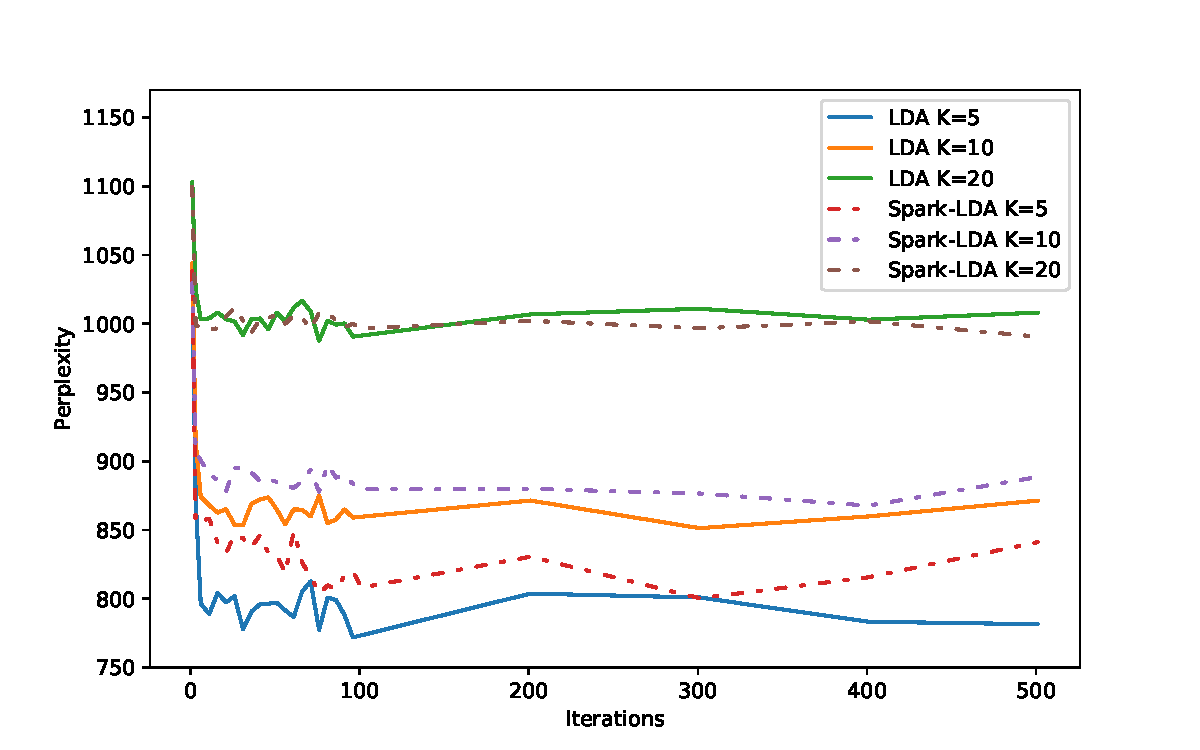
\includegraphics[scale=0.4]{plots/perplexity1.pdf}%
\label{fig:perplex2}}
\subfloat[NIPS abstracts]{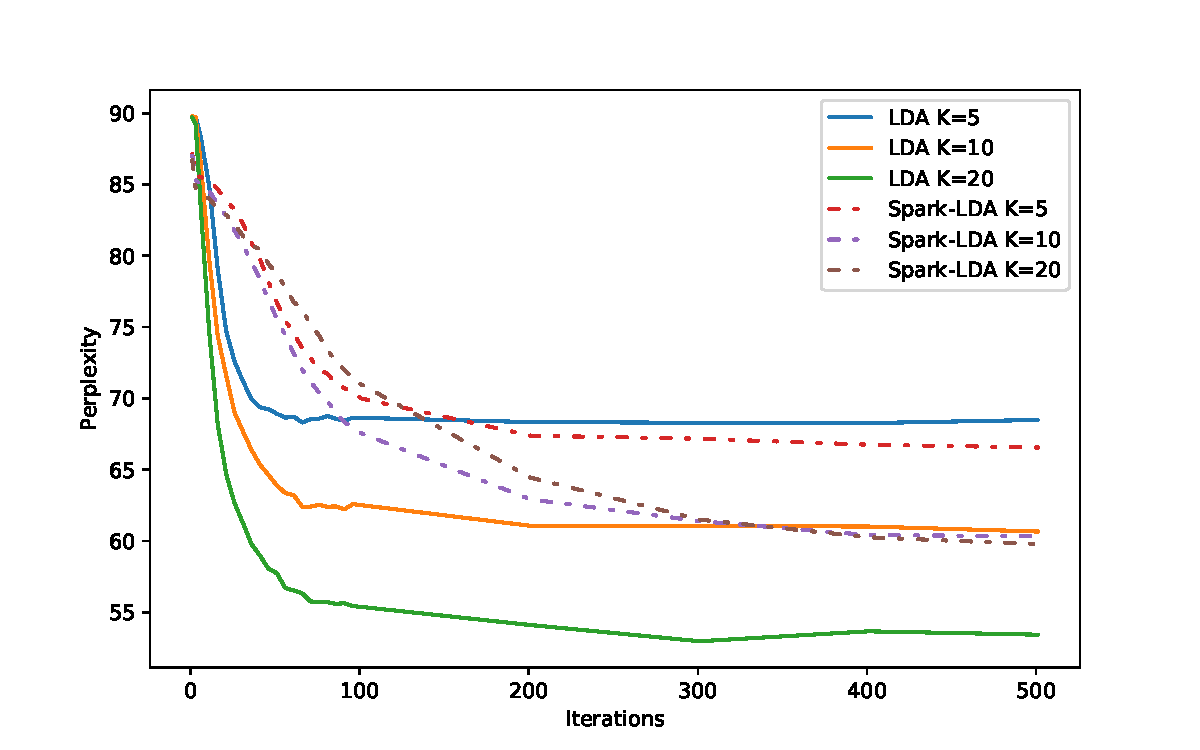
\includegraphics[scale=0.4]{plots/perplexity2.pdf}%
\label{fig:perplex2}}
\caption{Perplexity during training for different number of topics.}
\label{fig:sim}
\end{figure*}
The perplexity results for ABC News headlines S and NIPS abstracts, presented on Figure~\ref{fig:sim}, shows that Spark-LDA exhibits usually slower convergence rate than the sequential LDA algorithm, which is to be expected considering the fact that it relaxes the sequential sampling requirement. However, in most cases Spark-LDA is able to achieve very close or the same final perplexity value as the regular LDA model, but it requires more iterations. Note that when problem dimensions are increasing (e.g. the number of documents/topics/words), the distributed model requires more iterations to achieve model quality comparable to the sequential LDA, what can be observed with the difference in the convergence rate between two studied datasets.


\subsection{Execution time}

\renewcommand{\arraystretch}{1.2}
\begin{table*}[t]
\centering
\caption{Execution time in seconds and speedup achieved by Spark-LDA with respect to different number of topics.}
\begin{tabular}{lrrrrrrr} \toprule
                 & \multicolumn{3}{c}{\textbf{ABC News headlines S}} & \multicolumn{3}{c}{\textbf{NIPS abstracts}}        & \multicolumn{1}{c}{\textbf{ABC News headlines F}} \\
                 & K = 5             & K = 10           & K = 20           & K = 5           & K = 10          & K = 20         & K = 2                                           \\ \midrule
LDA              & 47,80             & 51,59            & 57,41            & 1 729,06        & 1 779,65        & 2 002,13       & 32 577,60                                       \\
Spark-LDA        & 117,27            & 126,82           & 143,06           & 128,03          & 159,32          & 207,01         & 3 929,08                                        \\ \midrule
\textbf{Speedup} & \textbf{0,408}    & \textbf{0,407}   & \textbf{0,401}   & \textbf{13,505} & \textbf{11,170} & \textbf{9,672} & \textbf{8,291}  \\ \bottomrule                         
\end{tabular}
\label{tab:speedup}
\end{table*}

Execution time and speedup for the distributed and sequential models with respect to three datasets and different number of topics is presented in Table~\ref{tab:speedup}. Overall, one can notice that using Spark-LDA for processing small     datasets results in increase of the execution time when compared to the regular LDA.  For the ABC News headlines S dataset, using Spark-LDA increased execution time nearly three times when compared to the sequential algorithm. Given the overhead of starting Spark context, data distribution and the time needed for the global count vales updates and broadcasts, Spark-LDA is unable to compete with the sequential LDA as, although it processes documents one by one, it does not require additional variables synchronization. The speedup and performance improvement  when using Spark-LDA can be observed only when this model is applied to medium and large datasets as the mentioned overhead is greatly reduced by the processing document in parallel. For NIPS abstracts dataset, the Spark-LDA model achieved speedup of 13.505, 11.170 and 9.672 for number of topic equal to 5, 10 and 20 respectively, while for the ABC News headlines F the distributed algorithm was about 8 times faster than the sequential model.

\subsection{Interval between updates}
One of the essential parameter influencing the model quality and time of training of Spark-LDA is the \textit{interval between updates} parameter. To evaluate the effect of this parameter, perplexity and execution time for the Spark-LDA model were measured when running the algorithm with values of the parameter equal to 5, 10, 20 and 50 iterations for ABC News headlines S and NIPS abstracts datasets. The results for perplexity metric are presented in Figure~\ref{fig:update-perplex}, and the comparison on the execution time is shown in Figure~\ref{fig:update-time}.  As expected, one can notice that increasing the value of the \textit{interval between updates} parameter causes decreasing the convergence rate, as the requirement of sequential sampling becomes strongly violated. However, increasing this value also decreases execution time since it limits the number of updates and broadcasts performed for the global count values. Additionally, it is also worth nothing that this problem arises with increasing dimensions of dataset, thus this parameter should be set up with value allowing to achieve a balance between model quality and execution time.

\begin{figure*}[t]
\centering
\subfloat[ABC News headlines S]{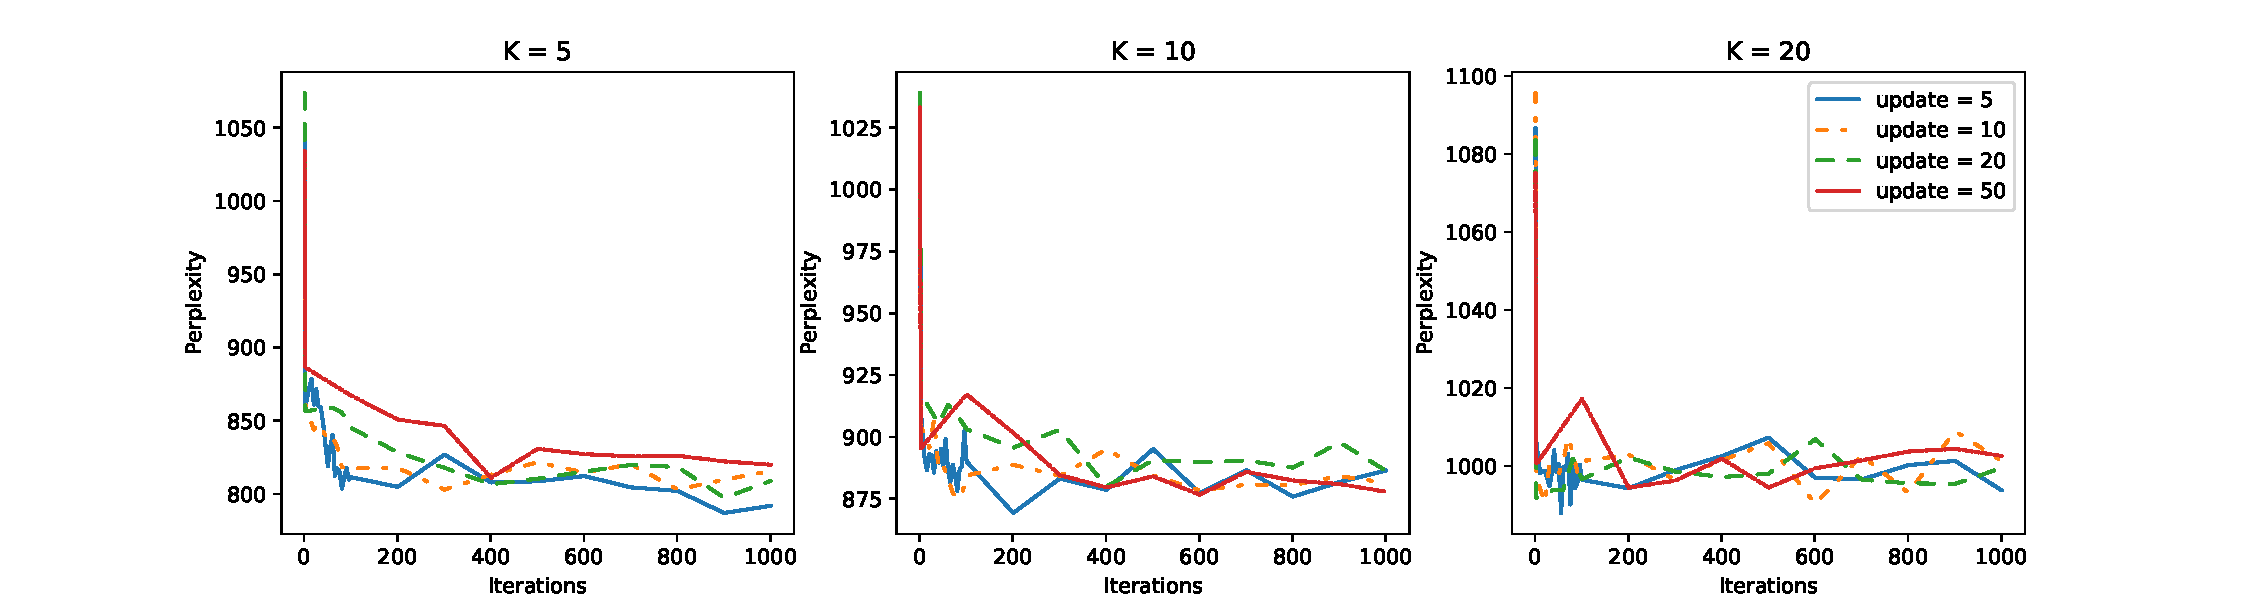
\includegraphics[scale=0.42]{plots/update_abc.pdf}%
\label{fig:param_abc}}
\hfil
\subfloat[NIPS abstracts]{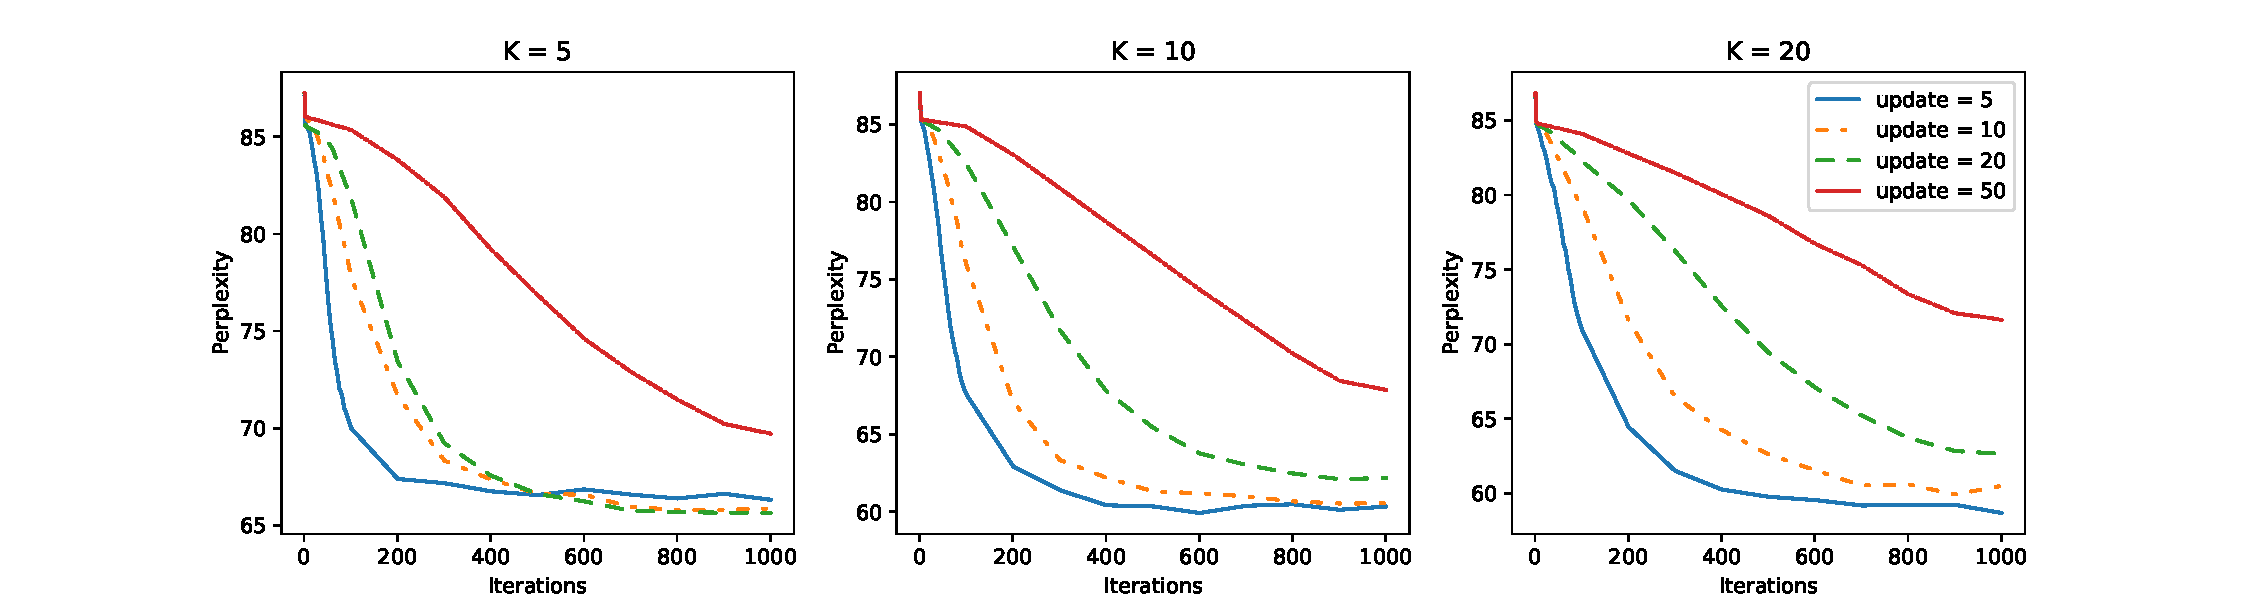
\includegraphics[scale=0.42]{plots/update_abstract.pdf}%
\label{fig:param_nips}}
\caption{Perplexity during training Spark-LDA for different values of the \textit{interval between updates} parameter.}
\label{fig:update-perplex}
\end{figure*}

\begin{figure*}[t]
\centering
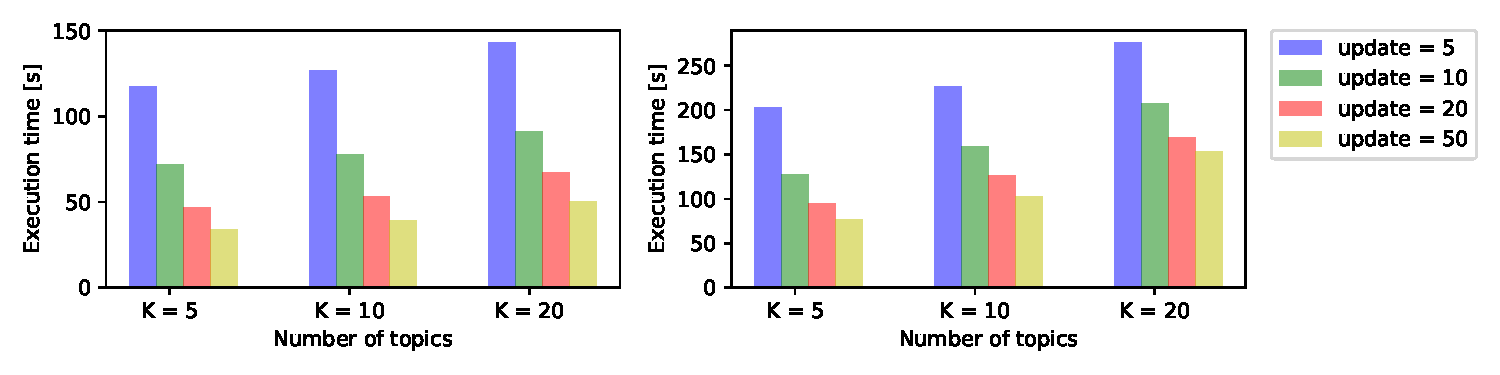
\includegraphics[scale=0.6]{plots/param_update.pdf}
\caption{Execution time of Spark-LDA on ABC News headlines S (left) and NIPS abstracts (right) with respect to the \textit{interval between updates} parameter.}
\label{fig:update-time}
\end{figure*}



\section{Conclusion}
\label{sec:conclusion}
This report provides a description of distributed collapsed Gibbs sampling for LDA implemented on Spark, Spark-LDA. The results of the experiments show that the proposed algorithm is able to achieve comparable results in terms of model quality when compared to the sequential LDA, while providing significant speedup due to using parallelized approximate Gibbs sampling procedure. However, the current implementation on Spark-LDA could be further improved by reducing the amount of data to be synchronized through a optimized partitioning and shuffling involving distribution of the data at the level of words.

\bibliographystyle{IEEEtran}
\bibliography{IEEEabrv,paper}


\end{document}


